\documentclass[11pt]{article}
\usepackage[table]{xcolor}
\usepackage[margin=1.0in]{geometry}
\usepackage{mathtools}
\usepackage{graphicx}
\usepackage{float}
\usepackage[font=small]{caption}
\usepackage{color}
\usepackage{fancyhdr}
%\usepackage{soul} %for striking out text
%\usepackage{arydshln} % for dotted line on truth table
\usepackage{tikz} % graphics stuff
\usepackage{caption}
\usepackage{gensymb}
\usepackage{booktabs}
\usepackage{listings}
\usepackage{fancyvrb}
\usepackage{amsmath}
%\usepackage{subcaption} % used to horizontally tile figures
%\usepackage{listings}
\pagestyle{fancy}
\fancyhead{}
\fancyfoot{}
\fancyfoot[R]{\thepage}


%\usepackage{xcolor}    % loads also »colortbl«


\definecolor{lightgray}{gray}{0.9}
\let\oldtabular\tabular
\let\endoldtabular\endtabular
\renewenvironment{tabular}{\rowcolors{2}{white}{lightgray}\oldtabular}{\endoldtabular}


\begin{document}


%
% cover page
%

\vspace*{6 cm}

\begin{center}
\bf{CMPE-655 Multiple Processor Systems\\
    Asignment 2\\
\vspace{0.25 cm}
Parallel Implementation of a Ray Tracer
}
\end{center}

\vspace{6 cm}

\begin{flushright}
Brandon Key\\
Submitted: 15 April 2020\\
\vspace{0.5 cm}
Instructor: Dr. Shaaban\\
TAs: Robert Mason \\
Adam Smith\\
Designed by: \\
\vspace{0.5 cm}
\end{flushright}



%\tableofcontents
\newpage

\section{Abstract}
	
	
	

\section{Design Methodology and Theory}

	The given sequential code was the basis for all partitioning methods. 
	
	The communication time for all methods was found by subtracting the computation time from the total execution time. This ensure that any hidden communication was not measured as would be the case if communication time was explicitly measured. Clock time was captured before and after processing. The difference represented the computation time. The longest computation among the slaves and master was considered the total system computation time since the system would be waiting on the slowest slave. 
	

	\subsection{Static Strips}
		The first partitioning scheme that was implemented was static vertical strips. Each processor was responsible for rendering an even share of the image as seen in Equation \ref{eqn:strip_size}.
		
		\begin{equation}\label{eqn:strip_size}
			Columns to Process = \frac{Image Width}{Number of Processors}
		\end{equation}
		\begin{center}
			Equation \ref{eqn:strip_size}: Strip Size
		\end{center}
	
		Since the calculation for strip size is integer based, there is a remainder. These remaining columns were given to the lowest ranked processors by giving those lowest ranked processors one extra column. Figure \ref{fig:strips} shows the division of the image to processors.
		
		\begin{figure}[H]
			\centering
			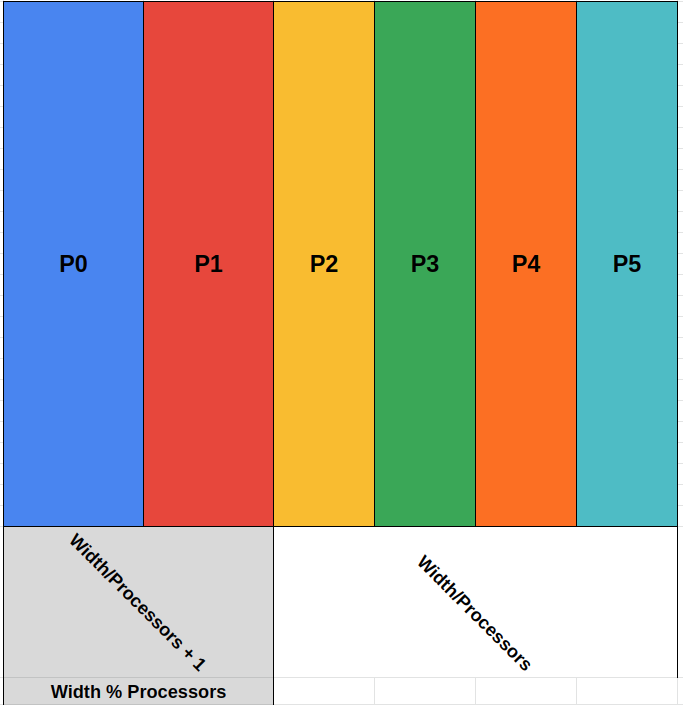
\includegraphics[width=0.7\linewidth]{Pictures/Strips}
			\caption{Static Vertical Strips}
			\label{fig:strips}
		\end{figure}
	
		The computation time also needed to be sent to the master along with the pixels. This was done by allocating an extra float to the end of the pixel array and appending the computation time there. The master would iterate through the slave ranks and accept the packet of pixels. The master would store the computation time if it was the largest one encountered and copy the pixels in the packet into the master packet array. 
		
		It should be noted that in order to facilitate vertical strips, the slaves represented the pixels in row major form so that computations happened in a contiguous memory. This at least allowed the pixel array to be in cache more often since there is more locality. 
	
	\subsection{Static Cycles}
	
		The next partition scheme was cyclical assignment. Instead of processors handling a contiguous strip of pixels, a processor handles a few rows of pixels at a time. Figure \ref{fig:cycles} shows how 4 processors would be responsible for calculations. 
		
		\begin{figure}[H]
			\centering
			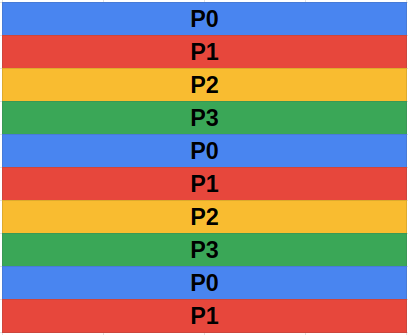
\includegraphics[width=0.7\linewidth]{Pictures/Cycles}
			\caption{Static Horizontal Cycles}
			\label{fig:cycles}
		\end{figure}
	
		It was determined that an iterative approach would best handle the required calculations; each processor would iterate over all rows, and check if it should process that row. Equation \ref{eqn:cycle_calc} shows the check that each processor performs to check if it should calculate the pixel value.
	
		\begin{equation}\label{eqn:cycle_calc}
		rank == \frac{row}{CycleSize} \% Processors
		\end{equation}
		\begin{center}
			Equation \ref{eqn:cycle_calc}: Rows Each Processor is Responsible For
		\end{center}
	
		An iterative approach simplifies design, and the check for row calculation is much less intensive than the calculation being performed, little performance is lost. This check naturally leads to the lower ranked tasks handling the "leftover" rows. Since the image cannot always be divided evenly by the cycle size, calculations are stopped when the row reaches image edge (via bounds of a for loop).
		
		When the master receives slave results, it must copy the rows from the packet into the pixel array. This was trivial as both the pixel array and the packet array had the same row width. While going through the packet, the master kept track of which row (from the slave perspective) it was on in order to reverse the logic that slave performed. At the end of the packet was the computation time again.
	
	\subsection{Static Blocks}
	
		The third partitioning scheme is static blocks. The image was broken into (nearly) equal size blocks. The number of blocks was determined by the number of processors available. The width of the image in blocks is the square root of the number of processors. Equation \ref{eqn:image_size_blk} shows the calculation of the width of the image in blocks. Note that the number of processors is limited to perfect squares.
		
		\begin{subequations}
		\begin{align}\label{eqn:image_size_blk}
			\text{Image Size (blocks)} & == \text{Image Width (blocks)} * \text{Image Height (blocks)}
			\\
			\text{Image Width (blocks)} & = \sqrt{\text{Image Size}}
			\\
			\text{Image Height (blocks)} & = \sqrt{\text{Image Size}}
		\end{align}
		\end{subequations}
		\begin{center}
			Equation \ref{eqn:image_size_blk}: Rows Each Processor is Responsible For
		\end{center}
	
		Figure \ref{fig:blocks} shows the division of the image between processors.
		
		\begin{figure}[H]
			\centering
			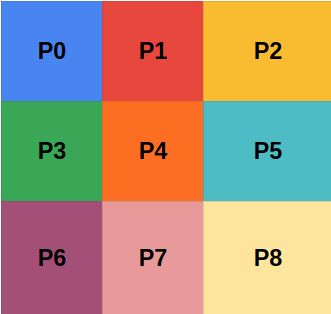
\includegraphics[width=0.7\linewidth]{Pictures/Blocks}
			\caption{Static Blocks}
			\label{fig:blocks}
		\end{figure}
	
		The figure shows that blocks on the end are not the same size as the blocks at the beginning. In order to accommodate the remainder of the pixels that results from dividing the image size by $\sqrt{Processors}$, the remaining pixels are given to the last n blocks. By putting the larger blocks closer to the end, it gives the master time to communicate and handle the data from the lower ranked slaves, which hopefully finisher quicker. 
		
		To facilitate computation, a struct the represents a block was created. It specifies the coordinates of block in terms of blocks and pixels. This allows easily determining the appropriate packet size as well as which pixels the tasks should process. This helped both slave and master as well as cleaned up the code. 
		
		Like with other static partitioning schemes, the master would receive slave packets in order of their rank. Again, the packet would contain the computation time of the slaves after the pixel data. The master stored the computation time if it was larger than the currently stored computation time. 
	
	\subsection{Dynamic Blocks}
	
		Dynamic partitioning was the final scheme that was implemented. Unlike the static partitioning schemes, processors were not assigned work at startup, instead, when a slave finishes a work unit, it requests a new job from the master. This means that the master is not responsible for rendering, and instead just accepts packets from slaves and delegates work. At startup, slaves take a work unit based on their rank. This was done to eliminate communication on startup. Since the master would have to talk to each slave one at a time at startup, this would cause a lot of un-masked communication. Instead of the master telling slaves which pixels to calculate, slaves were told which job id to work on next. This meant that slaves had to calculate their pixel range for each job. This is a few simple calculations which is hopefully quicker than the reduced communication as a result.
		
		The master would wait for a message from any slave. This packet would contain the resulting pixels as well as: slave computation time, slave rank, and the job id that was just completed. The slave rank was sent so that the master knew where to send the next job. The job id was included so that the master could work out where the pixels map into the master pixel array. Job id was incremented by one each time a new slave finished work. Before the packet was fully parsed, the next job id was send to the slave as soon as the slave id was parsed from the packet. This was done so that the slave wouldn't have to wait on the master to start working on the next job. Once the master was out of new jobs, the master went into a different state. 
		
		In this new state, the master would still receive new packets from any slave, but it would send -1 as the new job id to slaves. This would tell the slaves that there is no more work. In this new state, the master would start storing the longest computation time. The master would know that once it received a packet from each slave, all computation was done. 
		
		 The image was divided into blocks (work units) of user defined size. Figure \ref{fig:dynamic} shows an image divided up into blocks.
		
		\begin{figure}[H]
			\centering
			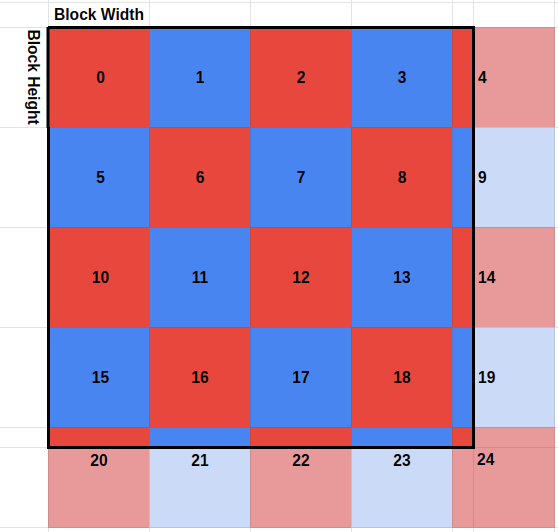
\includegraphics[width=0.7\linewidth]{Pictures/Dynamic}
			\caption{Dynamic Blocks}
			\label{fig:dynamic}
		\end{figure}
	
		When a block did not fit on the image, the block was clipped. In other schemes that would lead to load imbalance, but dynamic partitioning causes the slave to simply get a new job quicker. Blocks could be rectangular or square. 
	
\section{Results and Analysis}

	To test the performance of each partitioning scheme, each was tested with varying number of processors and various work sizes. The parallel implementations were compared to sequential 

	\subsection{Sequential}
		The sequential code took 112.94 seconds to parse the simple image and 3585.36 seconds to parse the complex image. 
		
		
	\subsection{Static Strips}
		
		Static vertical strips were divided among processors evenly, and there were no varying parameters other than processors. The performance when rendering the simple image was recorded in Table \ref{tab:strips_simple} and visualized in Figure \ref{fig:static-strips}.
		
		\begin{figure}[H]
			\centering
			\includegraphics[width=0.7\linewidth]{"Pictures/Static Strips"}
			\caption{Performance Scaling of Static Vertical Strips}
			\label{fig:static-strips}
		\end{figure}
	
		It can be seen that performance dramatically increases with more processors when there are few processors ($<$16). As more processors are dedicated to the problem, the performance increase decreases.
		
		\begin{table}[H]
			\caption{Performance of Vertical Strips with Simple Image}
			\label{tab:strips_simple}
			\centering
			\begin{tabular}{|c|c|c|c|c|}
				\multicolumn{5}{c}{\textbf{Static Strip Allocation}} \\
				\hline
				\textbf{Processes} & \textbf{Strips} & \textbf{Exec. Time (s)} & \textbf{Speedup} & \textbf{C-to-C ratio} \\
				\hline
				1 (srun -n 1)                    & 1         & 175.619535 & 0.643  & 0        \\
				2 (srun -n 2)                    & 2         & 121.061101 & 0.933  & 0.000505 \\
				4 (srun -n 4)                    & 4         & 82.225865  & 1.374  & 0.002754 \\
				9 (srun -n 9)                    & 9         & 41.130541  & 2.746  & 0.003184 \\
				16 (srun -n 16)                  & 16        & 26.236589  & 4.305  & 0.028886 \\
				20 (srun -n 20)                  & 20        & 22.363491  & 5.050  & 0.118175 \\
				25 (srun -n 25)                  & 25        & 18.112424  & 6.235  & 0.097723 \\
				36 (srun -n 36)                  & 36        & 12.570574  & 8.984  & 0.093093 \\
				49 (srun -n 49)                  & 49        & 10.159625  & 11.117  & 0.19525  \\
				55 (srun -n 55)                  & 55        & 9.505927   & 11.881  & 0.188241 \\
				64 (srun -n 64)                  & 64        & 8.895179   & 12.697  & 0.368489 \\
				\hline
			\end{tabular}
		\end{table}
	
		It should be noted that this algorithm is slower than the sequential code until 4 or more processors are used. An ideal speedup would match the number of processors, but it was noted that the speedup was about a quarter of the ideal speed. At 4 cores, a speedup of 1.374 was achieved, which is a bit more than a quarter of the ideal speedup of 4. At 36 cores, a speedup of 8.9 was realized, which is slightly less than the quarter of ideal speed up (9). The a quarter of ideal speedup at 64 processors would be 16, but only a speedup of 12.6 was achieved. This shows that not only is the speedup less than ideal, it becomes relatively less efficient with more processors. This is partially due to the increasing communication times. This is also partially due to the system being limited by the slowest processor. The more active processors, the greater the chance that another task from another user is slowing the machine.  
	
	\subsection{Static Cycles}
	
		Static Cycles has the parameters of: processors and cycle size. The simple image was rendered with 4, 9, and 16 processors for various cycle sizes. The results were recorded in Table \ref{tab:cycles_simple_cycle_size}. 

		\begin{table}[H]
			\caption{Performance of Horizontal Cycles with Simple Image as Cycle Size Varies}
			\label{tab:cycles_simple_cycle_size}
			\centering
			\begin{tabular}{|c|c|c|c|c|}
				\multicolumn{5}{c}{\textbf{Static Cyclical Allocation}} \\
				\hline
				\textbf{Processes} & \textbf{Strip Height (pixels)} & \textbf{Exec. Time (s)} & \textbf{Speedup} & \textbf{C-to-C ratio} \\
				\hline
				4 (srun -n 4)    & 1     & 47.654  & 2.370  & 0.011687  \\
				4 (srun -n 4)    & 5     & 47.649  & 2.370  & 0.004629  \\
				4 (srun -n 4)    & 10    & 47.672  & 2.369  & 0.011275  \\
				4 (srun -n 4)    & 20    & 47.873  & 2.359  & 0.00514   \\
				4 (srun -n 4)    & 80    & 48.269  & 2.340  & 0.01162   \\
				4 (srun -n 4)    & 320   & 49.859  & 2.265  & 0.005853  \\
				4 (srun -n 4)    & 640   & 52.365  & 2.157  & 0.005939  \\
				4 (srun -n 4)    & 1280  & 82.994  & 1.361  & 0.002594  \\
				9 (srun -n 9)    & 1     & 22.686  & 4.978  & 0.078114  \\
				9 (srun -n 9)    & 5     & 21.511  & 5.250  & 0.005657  \\
				9 (srun -n 9)    & 10    & 22.969  & 4.917  & 0.083974  \\
				9 (srun -n 9)    & 20    & 21.982  & 5.138  & 0.017573  \\
				9 (srun -n 9)    & 40    & 23.232  & 4.861  & 0.070674  \\
				9 (srun -n 9)    & 160   & 25.078  & 4.504  & 0.016896  \\
				9 (srun -n 9)    & 350   & 28.399  & 3.977  & 0.016553  \\
				9 (srun -n 9)    & 650   & 48.166  & 2.345  & 0.005191  \\
				16 (srun -n 16)  & 1     & 14.010  & 8.061  & 0.179885  \\
				16 (srun -n 16)  & 5     & 13.371  & 8.446  & 0.124782  \\
				16 (srun -n 16)  & 10    & 14.056  & 8.035  & 0.177079  \\
				16 (srun -n 16)  & 20    & 13.519  & 8.354  & 0.115796  \\
				16 (srun -n 16)  & 50    & 14.400  & 7.843  & 0.132413  \\
				16 (srun -n 16)  & 100   & 16.255  & 6.948  & 0.135441  \\
				16 (srun -n 16)  & 250   & 21.617  & 5.225  & 0.077393  \\
				16 (srun -n 16)  & 400   & 34.928  & 3.234  & 0.089348  \\
				\hline
			\end{tabular}
		\end{table}
	
		The performance when varying cycle size was plotted in Figure \ref{fig:cycles-strip-size}.
		
		\begin{figure}[H]
			\centering
			\includegraphics[width=0.7\linewidth]{"Pictures/Cycles Strip Size"}
			\caption{Performance Scaling of Cycle Size}
			\label{fig:cycles-strip-size}
		\end{figure}
	
		As strip size increases, so does load imbalance. This causes performance to decrease when strip size increases. 
		
		Once performance scaling with cycle size was known, the performance scaling with processor number was desired. As such, the cycle size was held constant at 27 and the number of processors were varied. The results were stored in Table \ref{tab:cycles_simple_procs}.
	
		\begin{table}[H]
			\caption{Performance of Horizontal Cycles with Simple Image as Number of Processors Varies}
			\label{tab:cycles_simple_procs}
			\centering
			\begin{tabular}{|c|c|c|c|c|}
				\multicolumn{5}{c}{\textbf{Static Cyclical Allocation}} \\
				\hline
				\textbf{Processes} & \textbf{Strip Height (pixels)} & \textbf{Exec. Time (s)} & \textbf{Speedup} & \textbf{C-to-C ratio} \\
				\hline
				1 (srun -n 1)    & 27  & 173.187  & 0.652   & 0         \\
				2 (srun -n 2)    & 27  & 89.103   & 1.268   & 0.002158  \\
				4 (srun -n 4)    & 27  & 48.128   & 2.347   & 0.005378  \\
				9 (srun -n 9)    & 27  & 24.305   & 4.647   & 0.131897  \\
				16 (srun -n 16)  & 27  & 13.658   & 8.269   & 0.120874  \\
				20 (srun -n 20)  & 27  & 14.311   & 7.892   & 0.394911  \\
				25 (srun -n 25)  & 27  & 10.655   & 10.599  & 0.328285  \\
				36 (srun -n 36)  & 27  & 10.214   & 11.057  & 0.723326  \\
				49 (srun -n 49)  & 27  & 8.846    & 12.768  & 1.087796  \\
				55 (srun -n 55)  & 27  & 12.878   & 8.770   & 2.074718  \\
				64 (srun -n 64)  & 27  & 7.341    & 15.384  & 0.927029  \\
				\hline
			\end{tabular}
		\end{table}
	
		To better visualize the data, Figure \ref{fig:cycles-cores} was created.
		
		\begin{figure}[H]
			\centering
			\includegraphics[width=0.7\linewidth]{"Pictures/Cycles Cores"}
			\caption{Performance Scaling with Increasing Number of Processors}
			\label{fig:cycles-cores}
		\end{figure}
	
		Performance of the static horizontal cycles matches the sequential code after 2 cores are given to rendering.  After 25 processors, the benefit of adding more processors is greatly reduced. With a more complex task, this may extend to more cores.
	
	\subsection{Static Blocks}
	
		The performance scaling of static blocks with increasing the number of processors was measured and recorded in Table \ref{tab:blocks_simple}. 
	
		\begin{table}[H]
			\caption{Performance of Blocks with Simple Image}
			\label{tab:blocks_simple}
			\centering
			\begin{tabular}{|c|c|c|c|c|}
				\multicolumn{5}{c}{\textbf{Static Block Allocation}} \\
				\hline
				\textbf{Processes} & \textbf{Blocks} & \textbf{Exec. Time (s)} & \textbf{Speedup} & \textbf{C-to-C ratio} \\
				\hline
				1 (srun -n 1)    & 1   & 179.020  & 0.631 & 0        \\
				4 (srun -n 4)    & 4   & 74.761   & 1.511 & 0.01028  \\
				9 (srun -n 9)    & 9   & 55.282   & 2.043 & 0.073443 \\
				16 (srun -n 16)  & 16  & 35.953   & 3.141 & 0.027227 \\
				25 (srun -n 25)  & 25  & 22.797   & 4.954 & 0.139857 \\
				36 (srun -n 36)  & 36  & 21.581   & 5.233 & 0.166538 \\
				49 (srun -n 49)  & 49  & 18.009   & 6.271 & 0.334002 \\
				64 (srun -n 64)  & 64  & 15.210   & 7.425 & 0.267504 \\
				\hline
			\end{tabular}
		\end{table}
	
		Performance scaling was graphed in Figure \ref{fig:blocksscaling}.
		
		\begin{figure}[H]
			\centering
			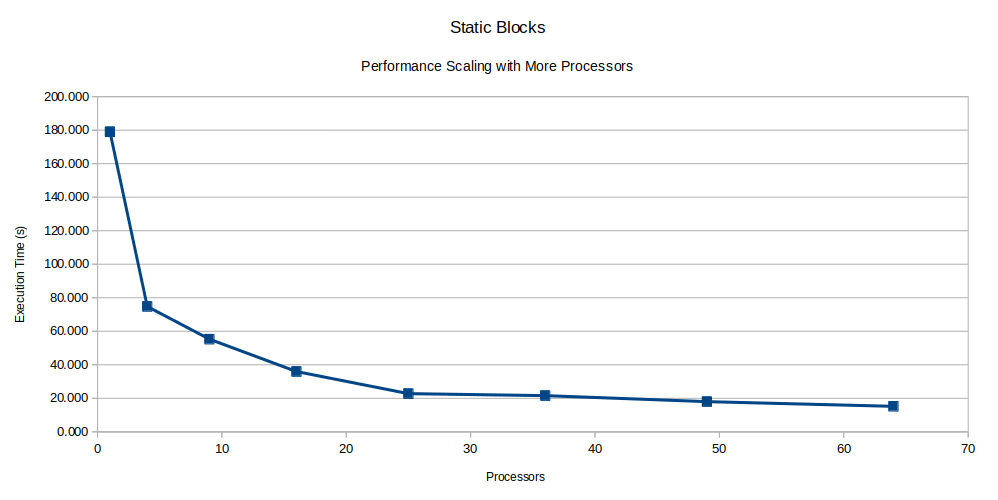
\includegraphics[width=0.7\linewidth]{Pictures/blocks_scaling}
			\caption{Performance of Static Blocks with Simple Image as Number of Processors Varies}
			\label{fig:blocksscaling}
		\end{figure}
	
		This partitioning scheme doesn't match the speed of the sequential code until there are 4 processors being used. It also seems the block partitioning is slower than the other static partitioning methods. This is likely due to the poor locality of the data. While a block is spatially local in an image, the image is represented as a 1D array in memory. Jumping between rows causes the cache to need to reload pixel data. 
	
		
	
	\subsection{Dynamic Blocks}
	
		To examine the performance of dynamic blocks, multiple square block sizes were tested with 9 and 16 processors. The results were stored in Table \ref{tab:dynamic_square}.
	
		\begin{table}[H]
			\caption{Performance of Blocks - Simple Image with Square Blocks}
			\label{tab:dynamic_square}
			\centering
			\begin{tabular}{|c|c|c|c|c|}
				\multicolumn{5}{c}{\textbf{Dynamic Allocation}}        \\
				\hline
				\textbf{Processes} & \textbf{Block Size (rows x cols)} & \textbf{Exec. Time (s)} & \textbf{Speedup} & \textbf{C-to-C Ratio} \\
				\hline
				9 (srun -n 9)   & 1x1     & 38.433  & 2.939 & 7.30E-07 \\
				9 (srun -n 9)   & 15x15   & 25.908  & 4.359 & 7.94E-07 \\
				9 (srun -n 9)   & 25x25   & 26.083  & 4.330 & 9.49E-07 \\
				9 (srun -n 9)   & 50x50   & 23.540  & 4.798 & 1.10E-06 \\
				9 (srun -n 9)   & 75x75   & 24.575  & 4.596 & 1.10E-06 \\
				9 (srun -n 9)   & 100x100 & 23.523  & 4.801 & 1.00E-06 \\
				16 (srun -n 16) & 1x1     & 25.339  & 4.457 & 1.20E-07 \\
				16 (srun -n 16) & 15x15   & 14.009  & 8.062 & 1.37E-06 \\
				16 (srun -n 16) & 25x25   & 14.461  & 7.810 & 1.98E-06 \\
				16 (srun -n 16) & 50x50   & 14.185  & 7.962 & 1.45E-06 \\
				16 (srun -n 16) & 75x75   & 13.549  & 8.336 & 2.02E-06 \\
				16 (srun -n 16) & 100x100 & 12.938  & 8.729 & 1.54E-06 \\
				\hline
			\end{tabular}
		\end{table}
	
		
		To visualize the scaling, Figure \ref{fig:dynamic-simple} was created.
	
		\begin{figure}[H]
			\centering
			\includegraphics[width=0.7\linewidth]{"Pictures/Dynamic Simple"}
			\caption{Performance Scaling of Dynamic Mapping Processing Simple Image}
			\label{fig:dynamic-simple}
		\end{figure}
	
		With a work size of a single pixel, much time is wasted communicating and loading processor cache. It is interesting to note that the communication to computation ratio is still low at the block size of 1x1. This is likely due to the precision of floating points, where the calculation takes so little time that it is difficult to measure. Once a larger block size is used, performance doesn't change much with increasing block size, but performance does increase slightly with increasing block size.
		
		The performance when changing the shape of the blocks was recorded in Table \ref{tab:dynamic_oblong}.
	
		\begin{table}[H]
			\caption{Performance of Blocks - Simple Image with Oblong Blocks}
			\label{tab:dynamic_oblong}
			\centering
			\begin{tabular}{|c|c|c|c|c|}
				\multicolumn{5}{c}{\textbf{Dynamic Allocation}}      \\
				\hline
				\textbf{Processes} & \textbf{Block Size (rows x cols)} & \textbf{Exec. Time (s)} & \textbf{Speedup} & \textbf{C-to-C Ratio} \\
				\hline
				16 (srun -n 16) & 1x11  & 31.751 & 3.557  & 1.04E-06 \\
				16 (srun -n 16) & 10x1  & 37.412 & 3.019  & 5.17E-07 \\
				16 (srun -n 16) & 13x7  & 15.367 & 7.350  & 2.26E-06 \\
				16 (srun -n 16) & 29x5  & 15.644 & 7.219  & 1.19E-06 \\
				16 (srun -n 16) & 110x9 & 13.726 & 8.228  & 1.99E-06 \\
				16 (srun -n 16) & 1x70  & 16.945 & 6.665  & 1.13E-06 \\
				36 (srun -n 36) & 1x11  & 46.007 & 2.455  & 3.24E-07 \\
				36 (srun -n 36) & 10x1  & 49.738 & 2.271  & 3.08E-07 \\
				36 (srun -n 36) & 13x7  & 8.391  & 13.460 & 3.18E-06 \\
				36 (srun -n 36) & 29x5  & 8.282  & 13.636 & 2.33E-06 \\
				36 (srun -n 36) & 110x9 & 6.521  & 17.320 & 4.19E-06 \\
				36 (srun -n 36) & 1x70  & 10.135 & 11.144 & 2.23E-06 \\
				\hline
			\end{tabular}
		\end{table}
	
		Larger blocks seem to result in faster execution with the dynamic partitioning scheme.
	
		The measurements were repeated with the complex scene and recorded in Table \ref{tab:dynamic_square_complex}.
	
		\begin{table}[H]
			\caption{Performance of Blocks - Complex Image with Square Blocks}
			\label{tab:dynamic_square_complex}
			\centering
			\begin{tabular}{lllll}
				\multicolumn{5}{c}{\textbf{Dynamic Allocation}}        \\
				\hline
				\textbf{Processes} & \textbf{rows x cols} & \textbf{Exec. Time (s)} & \textbf{Speedup} & \textbf{C-to-C Ratio} \\
				\hline
				9 (srun –n 9)   & 1x1     & 752.421 & 4.765 & 3.51E-08 \\
				9 (srun –n 9)   & 15x15   & 742.651 & 4.828 & 2.38E-08 \\
				9 (srun –n 9)   & 25x25   & 764.933 & 4.687 & 2.05E-08 \\
				9(srun –n 9)    & 50x50   & 810.189 & 4.425 & 1.91E-08 \\
				9 (srun –n 9)   & 75x75   & 796.143 & 4.503 & 2.05E-08 \\
				9 (srun –n 9)   & 100x100 & 856.743 & 4.185 & 1.96E-08 \\
				16 (srun –n 16) & 1x1     & 827.368 & 4.333 & 2.48E-08 \\
				16 (srun –n 16) & 15x15   & 405.382 & 8.844 & 3.36E-08 \\
				16 (srun –n 16) & 25x25   & 437.604 & 8.193 & 3.59E-08 \\
				16 (srun –n 16) & 50x50   & 465.604 & 7.700 & 3.30E-08 \\
				16 (srun –n 16) & 75x75   & 467.381 & 7.671 & 3.95E-08 \\
				16 (srun –n 16) & 100x100 & 483.416 & 7.417 & 3.25E-08 \\
				\hline
			\end{tabular}
		\end{table}
	
		Again, the complex image rendering performance was visualized in Figure \ref{fig:dynamic-complex}.
	
		\begin{figure}[H]
			\centering
			\includegraphics[width=0.7\linewidth]{"Pictures/Dynamic Complex"}
			\caption{Performance Scaling of Dynamic Mapping Processing Complex Image}
			\label{fig:dynamic-complex}
		\end{figure}
	
		The complex image scales the same as the simple image.
		
		Oblong block size was tested and recorded in Table \ref{tab:dynamic_oblong_complex}.
	
		\begin{table}[H]
			\caption{Performance of Blocks - Complex Image with Oblong Blocks}
			\label{tab:dynamic_oblong_complex}
			\centering
			\begin{tabular}{|c|c|c|c|c|}
				\multicolumn{5}{c}{\textbf{Dynamic Allocation}}       \\
				\hline
				\textbf{Processes} & \textbf{rows x cols} & \textbf{Exec. Time (s)} & \textbf{Speedup} & \textbf{C-to-C Ratio} \\
				\hline
				16 (srun –n 16) & 1x11  & 413.590 & 8.669  & 4.87E-08 \\
				16 (srun –n 16) & 10x1  & 411.836 & 8.706  & 6.49E-08 \\
				16 (srun –n 16) & 13x7  & 398.067 & 9.007  & 3.97E-08 \\
				16 (srun –n 16) & 29x5  & 400.791 & 8.946  & 3.91E-08 \\
				16 (srun –n 16) & 110x9 & 433.408 & 8.272  & 4.08E-08 \\
				16 (srun –n 16) & 1x70  & 398.639 & 8.994  & 2.24E-07 \\
				36 (srun –n 36) & 1x11  & 200.745 & 17.860 & 9.14E-08 \\
				36 (srun –n 36) & 10x1  & 240.474 & 14.910 & 8.40E-08 \\
				36 (srun –n 36) & 13x7  & 176.629 & 20.299 & 9.01E-08 \\
				36 (srun –n 36) & 29x5  & 181.390 & 19.766 & 9.16E-08 \\
				36 (srun –n 36) & 110x9 & 214.380 & 16.724 & 9.30E-08 \\
				36 (srun –n 36) & 1x70  & 172.041 & 20.840 & 1.06E-07 \\
				\hline
			\end{tabular}
		\end{table}
	
		It seems that having a block that is taller than it is wide causes performance loss. 
		

	\subsection{Comparing Schemes}
	
		In order to compare partitioning schemes, the best speedup with 16 processors was graphed in Figure \ref{fig:comparison}.
		
		\begin{figure}[H]
			\centering
			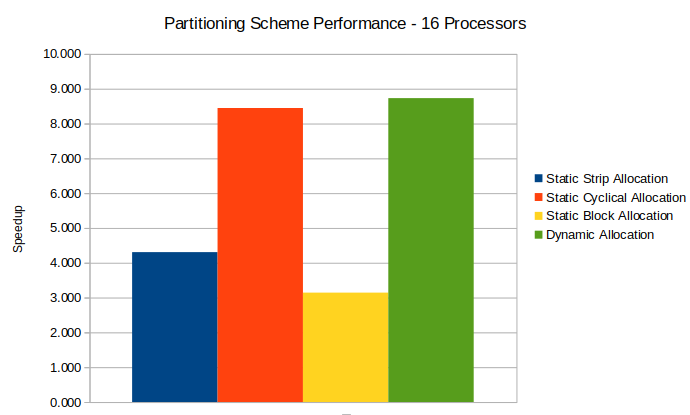
\includegraphics[width=0.7\linewidth]{Pictures/Comparison}
			\caption{Best Speedup with 16 Processors}
			\label{fig:comparison}
		\end{figure}
	
		Static cycles with a small cycle size was the fastest static partitioning scheme, while dynamic was faster yet dynamic was based off of blocks, which proved to be the slowest. If the dynamic mapping was combined with the cyclical partitioning scheme, it seems to reason that this would yield the fastest algorithm of this style.

\section{Conclusion}

	Since dynamic allocation was the last implementation, many lessons were learned during its implementation that could be applied to the static partitioning methods. In all static methods, the master waited for slave results in order of their rank. This causes blocking behavior if a slave with lower rank takes longer to finish processing than a slave with higher rank. To fix this, the master should accept results from any salve, and the slave number should have been included in the packet. Additionally, the master should be given the least amount of processing so it has time to process the slave results. 
	
	If there was more time to work on this project, it would have been useful to graph the load balancing of each processor. This could be done by having the master store all computation times of each slave and display them at the end. This could highlight load imbalance due to the partitioning scheme, non-homogeneous processors, or outside load on processors. 

	The static partitioning schemes try to balance load by giving each processor equal amounts of work. This works well if processors are homogeneous and only the ray-tracing program is running on the processors. If one processor is significantly faster (or less loaded) than the rest, it will sit idle, the converse is true too: a slower processor (or a more highly loaded one) will hold up the rest of the processors. Dynamic scheduling may have extra overhead in terms of the master not doing work and additional communication, but the more even load balancing tends to hide this overhead. The greater the difference in processors, the greater the advantage that dynamic scheduling will have.
	
	Overall, this project was useful in highlighting the importance of work distribution in a multi-processor application as well as the diminishing returns of adding more processors to a job. It was found that all of the parallel algorithms required 2 or more processors to match the performance of sequential code; only large jobs than can leverage multiple processors are worth parallelizing. 

\section{Acknowledgments}
	

\end{document}
